\section{Semantic Analysis} \label{sec:semantic-analysis}

Besides paper metadata and citation information, the text content of a document is another important source of information for recommender systems \cite{BaiScientificPaper2020,NascimentoSourceIndependent2011}. This section introduces the concept of embeddings to represent the document's content in numerical form that can be processed by language models. Based on these embeddings, the semantic similarity between documents can be computed, which is a key component of content-based recommender systems.

A \emph{token} in \ac{NLP} refers to a piece of a whole, so a token could correspond to a word, a subword, or even punctuation depending on how tokenization is performed. Although \emph{token} is more precise than \emph{word} from a technical perspective, the latter is still used in established terminology such as \emph{Word Embedding}, \emph{\acl{BoW}}, and \emph{Word2Vec}. Therefore, the terms are used interchangeably in this thesis.


\subsection{Embeddings} \label{sec:embeddings}

A core challenge in \ac{NLP} is converting the high-dimensional and non-numeric textual data into a format that computers can handle. To address this, various techniques have been developed for transforming, or \emph{embedding}, textual data into numeric vectors. These vectors capture the meaning of the language, making it possible for computational models to process it \cite{JurafskySpeechLanguage2022}.

Embeddings turn the separate and categorical aspects of text into a continuous, high-dimensional space. This space, known as the \emph{embedding space}, is organized to reflect the semantic and syntactic relationships between words \cite{MikolovEfficientEstimation2013}. In the embedding space, words with similar meanings or syntactic features are positioned close together, while dissimilar words are farther apart. This organization allows computational models to understand and process the meaning of text.

\Cref{fig:word-embeddings} illustrates an exemplary embedding space projected onto two dimensions. Words with similar meanings are placed closer together. Since the embedding task is inherently unsupervised, the word categories indicated by the different colors are not known in advance. Instead, they are discovered by the projection of the embedding space itself.
Similarly, cluster labels, such as \emph{Recommender Systems}, \emph{Language Models}, or \emph{Metrics} can be added after the fact for visualization purposes, but they are not available to the model during training.

\begin{figure}[ht]
    \centering
    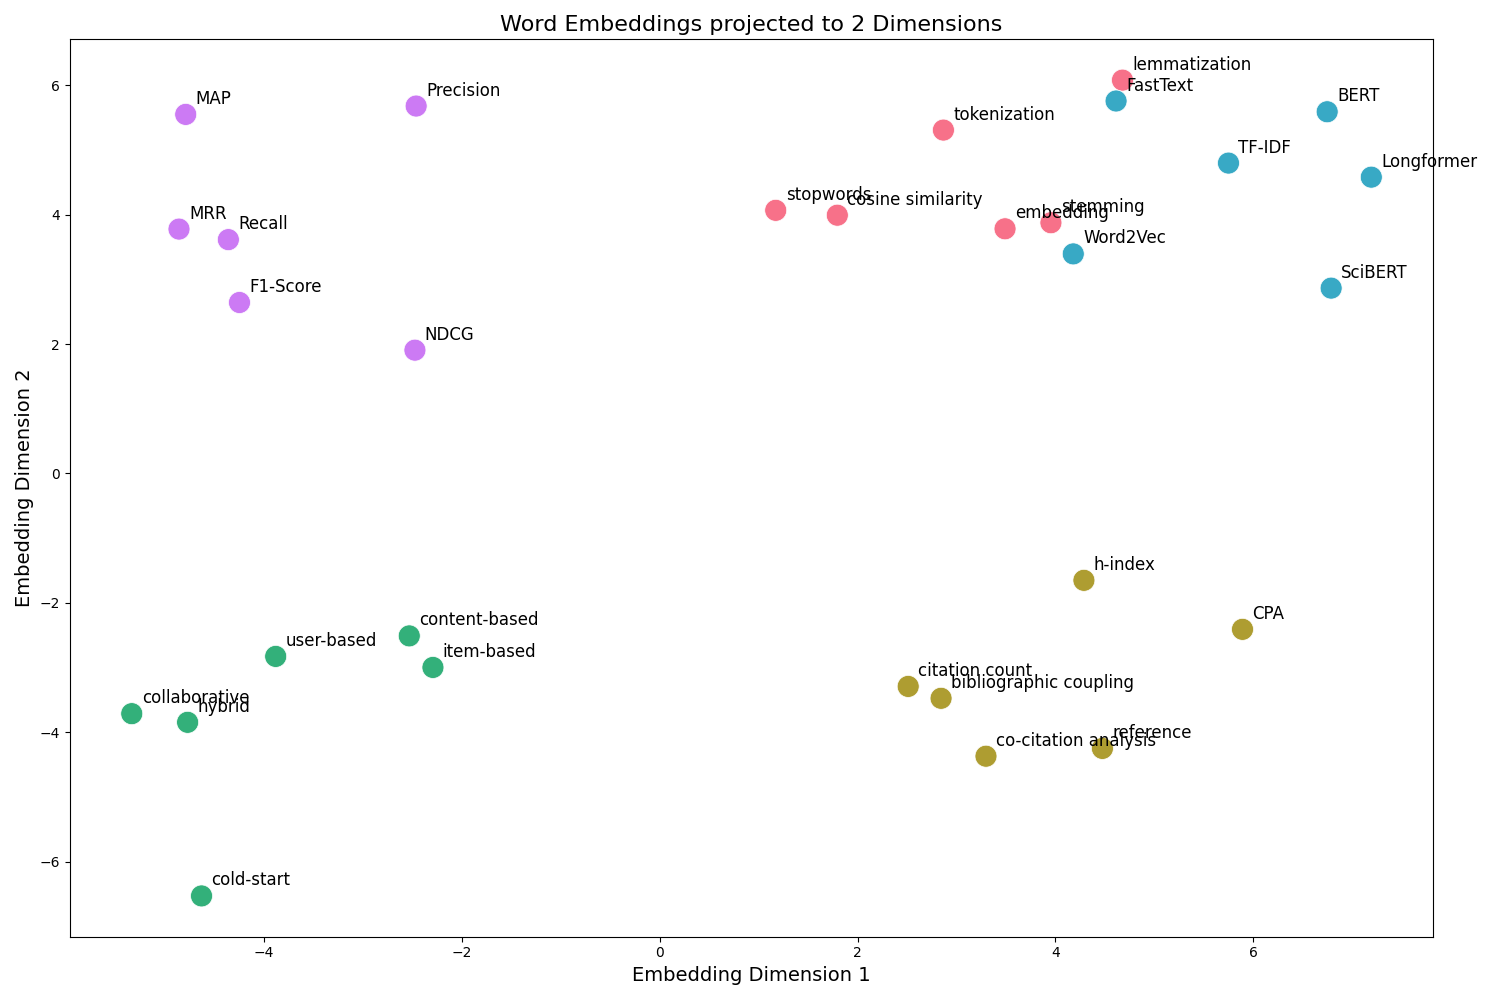
\includegraphics[width=0.9\textwidth]{plots/word_embeddings.png}
    \caption[The Embedding Space]{Conceptual visualization of the Embedding Space projected onto two dimensions. Words with similar meanings are placed closer together in the embedding space. The colors indicating word categories are added after the fact for visualization purposes and are not available to the model during training. The data for this figure was generated for illustration purposes and does not represent the embedding space of any specific model.}
    \label{fig:word-embeddings}
\end{figure}

Word embedding models typically rely on the distributional hypothesis \cite{HarrisDistributionalStructure1954} as their theoretical foundation. This hypothesis suggests that words used in similar contexts tend to have similar meanings \cite{JurafskySpeechLanguage2022}. The term \emph{context} can be defined in various ways. One popular approach uses a sliding window to define the context. The words that surround the target word within this window are considered its context. The window size is a hyperparameter of the model that can be tuned to achieve optimal results.

Learning word embeddings is an unsupervised task, meaning the model learns from raw text without needing explicit semantic or syntactic annotations. This makes them highly scalable and suitable for handling large bodies of text. On the flip side, this implies that embedding models generally cannot capture metadata not contained in the raw text, like the part-of-speech or grammatical role of a word.

After training, an embedding model can map any word in its vocabulary into the embedding space. However, words not in its vocabulary, known as \ac{OOV} words, can pose a challenge. This scenario regularly occurs when pretrained models are used on a different text corpus during inference. To address this, two common approaches are used. The first is to simply ignore \ac{OOV} words. In this case the unknown tokens do not impact the document embedding. The second approach is to map all \ac{OOV} words to a special token, such as \texttt{<UNK>}, and train the model to learn a representation for this token in the same way as for any other word \cite{JurafskySpeechLanguage2022}.

Numerous methods exist for generating numerical embedding vectors from text tokens. These methods can be broadly classified into two categories: \emph{sparse embeddings} and \emph{dense embeddings}.

\subsection{Sparse Embeddings} \label{sec:sparse-embeddings}

Sparse vector embeddings belong to a class of text representation models that employ a count-based vector space model. A key advantage of sparse embeddings lies in their interpretability: each dimension corresponds to a unique word from the vocabulary, and the value along that dimension indicates the significance of that word within the document: The higher the frequency of the word, the higher the relevance of that word to the document. This makes sparse vector embeddings a popular choice for tasks like document classification and information retrieval \cite{ManningIntroductionInformation2008,JurafskySpeechLanguage2022}.

The \ac{BoW} model represents the most basic form of sparse vector embeddings. Within the \ac{BoW} model, each document is depicted as a vector within an $N$-dimensional space, where $N$ denotes the size of the vocabulary. Each dimension is associated with a unique word from the vocabulary, and the value along that dimension reflects the count of that word within the document. Although this model is simple and efficient, it treats each word independently and fails to capture the order of the words within the document.

\subsubsection*{TF-IDF}

A more advanced form of sparse vector embeddings is the Term Frequency - Inverse Document Frequency (TF-IDF) model \cite{SaltonTermWeighting1987}. TF-IDF is a statistical measure that assesses the importance of a word to a document within a collection of documents. Unlike the simple count-based measure used in the \ac{BoW} model, TF-IDF considers not just the frequency of the word within the document (the term frequency), but also how common the word is across all documents in the corpus (the document frequency).

The TF-IDF model offers the benefit of down-weighting tokens common across all documents, such as stop words, while highlighting tokens unique to a specific document. This makes it more effective than the \ac{BoW} model at capturing the semantics of the document. The underlying assumption is that a term occuring in many documents is a less accurate discriminator than a term occuring in a small subset of documents and thus should be given less weight \cite{BreitingerAcademicLiterature2023}.

The TF-IDF score for a token $t$ within a document $d$ from a corpus $D$ can be calculated using the formula:

\begin{align}
    \text{tf-idf}(t, d, D) = \text{tf}(t, d) \cdot \text{idf}(t, D) \label{eq:tf-idf}
\end{align}

where $\text{tf}(t, d)$ is the term frequency of $t$ in $d$, and $\text{idf}(t, D)$ is the inverse document frequency of $t$ in $D$. The term frequency $\text{tf}(t, d)$ is typically the raw count of $t$ in $d$, although other measures such as the relative frequency are also employed. The inverse document frequency $\text{idf}(t, D)$ quantifies how common or rare $t$ is across all documents in $D$.

The precise formulas for the term frequency and inverse document frequency can vary. For example, Jurafsky and Martin \cite{JurafskySpeechLanguage2022} compute the term frequency using a logarithm with base 10:

\begin{align}
    \text{tf}(t, d) = \log_{10} \left( 1 + \text{count}(t, d) \right) \label{eq:tf}
\end{align}

where $\text{count}(t, d)$ is the number of occurrences of $t$ in $d$.

The rationale for incorporating the logarithm is that "a word appearing 100 times in a document doesn’t make that word 100 times more significant to the meaning of the document" \cite{JurafskySpeechLanguage2022}. A constant 1 is added to compute the logarithm for words that do not appear in the document (i.e., with a count of 0).

The inverse document frequency is computed by Jurafsky and Martin as

\begin{align}
    \text{idf}(t, D) = \log_{10} \left( \frac{|D|}{|\{d \in D : t \in d\}|} \right) \label{eq:idf}
\end{align}

where $|D|$ is the total number of documents in the corpus, and $|\{d \in D : t \in d\}|$ is the number of documents in which $t$ appears.

While the impact of slight variations in \Cref{eq:tf} and \Cref{eq:idf} for term frequency and inverse document frequency is often negligible, it is worth noting that the widely used \emph{scikit-learn} \cite{PedregosaScikitlearnMachine2011} implementation of the TF-IDF model defines the term frequency as

\begin{align}
    \text{tf}(t, d) = \text{count}(t, d) \label{eq:tf-sklearn}
\end{align}

and the inverse document frequency as

\begin{align}
    \text{idf}(t, D) = \log \left( \frac{1 + |D|}{1 + |\{d \in D : t \in d\}|} \right) + 1 \label{eq:idf-sklearn}
\end{align}

where $\log$ is the natural logarithm with base $e$. A constant 1 is added to the denominator of the inverse document frequency to prevent division by zero.


\subsubsection*{BM25 and BM25+}

BM25 is a ranking function employed in information retrieval systems that builds upon the TF-IDF model with several refinements \cite{RobertsonOkapiTREC31995}. The primary improvements include the addition of a document length normalization factor and a term frequency saturation factor. Both are designed to improve the robustness of the scoring mechanism, preventing overly frequent words from dominating the score and accounting for variations in document length.

The BM25 score for a token $t$ within a document $d$ from a corpus $D$ is computed using the formula:

\begin{align}
    \text{BM25}(t, d, D) = \text{BM25}_{tf}(t, d) \cdot \text{BM25}_{idf}(t, D) \label{eq:bm25}
\end{align}

where $\text{BM25}_{tf}(t, d)$ denotes the term frequency component of the BM25 score, and $\text{BM25}_{idf}(t, D)$ represents the inverse document frequency component of the BM25 score.

In the BM25 model, Robertson et al. \cite{RobertsonOkapiTREC31995} define the term frequency component as

\begin{align}
    \text{BM25}_{tf}(t, d) = \frac{(k_1 + 1) \cdot \text{tf}(t, d)}{k_1 \cdot ((1 - b) + b \cdot \frac{|d|}{avgdl}) + \text{tf}(t, d)} \label{eq:bm25-tf}
\end{align}

and the inverse document frequency component as

\begin{align}
    \text{BM25}_{idf}(t, D) = \log \left( \frac{|D| - |\{d \in D : t \in d\}| + 0.5}{|\{d \in D : t \in d\}| + 0.5} \right) \label{eq:bm25-idf}
\end{align}

where $k_1 > 0$ and $b \in [0, 1]$ are free parameters, $|d|$ indicates the length of the document $d$, and $avgdl$ is the average document length in the corpus \cite{RobertsonOkapiTREC31995}.

The $b$ parameter manages the length normalization. If $b = 0$,

\begin{align}
    (1 - b) + b \cdot \frac{|d|}{avgdl} = 1 \label{eq:bm25-b-0}
\end{align}

resulting in no length normalization.
If $b = 1$,

\begin{align}
    (1 - b) + b \cdot \frac{|d|}{avgdl} = \frac{|d|}{avgdl} \label{eq:bm25-b-1}
\end{align}

decreasing $\text{BM25}_{tf}$ for long document with $|d| > avgdl$ in \Cref{eq:bm25-tf}.
The length normalization ensures that long documents do not disproportionately benefit due to their size.

The $k_1$ parameter regulates the saturation of $\text{BM25}_{tf}(t, d)$. When $k_1$ approaches zero, $\text{BM25}_{tf}(t, d)$ gravitates towards one, which means that both $\text{BM25}_{tf}(t, d)$ and $tf(t, d)$ have minimal impact on the BM25 score as seen in \Cref{eq:bm25}.
Conversely, a large value of $k_1$ causes $\text{BM25}_{tf}(t, d)$ to be acutely sensitive to fluctuations in $tf(t, d)$ when $tf(t, d)$ is low. This is because the contribution of $tf(t, d)$ to the denominator in \Cref{eq:bm25-tf} is relatively minor in this range. As $tf(t, d)$ increases, the influence of any additional rise in term frequency begins to diminish, leading to a saturation effect for $\text{BM25}_{tf}(t, d)$.

BM25+ \cite{LvLowerboundingTerm2011}, an extension of BM25, sets a lower bound for the contribution of infrequent terms to the BM25 score by adding a constant $\delta > 0$:

\begin{align}
    \text{BM25+}_{tf}(t, d) = \text{BM25}_{tf}(t, d) + \delta \label{eq:bm25+-tf}
\end{align}

This adjustment aims to amplify the influence of rare terms on the BM25 score, ensuring that "even a single occurrence of a search term contributes at least a constant amount" to this score \cite{TrotmanImprovementsBM252014}. A frequently used value for $\delta$ is 1.0 \cite{LvLowerboundingTerm2011}.


\subsection{Dense Embeddings} \label{sec:dense-embeddings}

While sparse word embeddings are effective, they are inherently high-dimensional. Their dimensionality is equivalent to the size of the vocabulary, which results in a large number of dimensions, most of which have a value of zero.
This makes the representation rather inefficient, especially for extensive vocabularies \cite{ManningIntroductionInformation2008,JurafskySpeechLanguage2022}.

In contrast, dense word embeddings provide a more condensed representation. They map words into a lower-dimensional space, often in the range of hundreds or thousands of dimensions, where all dimensions carry information and have non-zero values \cite{MikolovEfficientEstimation2013, PenningtonGloveGlobal2014, BojanowskiEnrichingWord2017}. This compactness not only enhances computational efficiency but also improves the model's capacity to capture semantic and syntactic relationships between words \cite{MikolovEfficientEstimation2013, PenningtonGloveGlobal2014}.
In contrast to keyword-based sparse word embeddings, dense word embeddings are able to detect semantic similarity even in the absence of lexical overlap.

A key distinction between dense and sparse word embeddings lies in their learning mechanism. Sparse word embeddings are typically derived from explicit counts or statistics of the text data (e.g., term frequency in TF-IDF). In contrast, dense word embeddings are learned in an unsupervised fashion from large-scale text data \cite{ManningIntroductionInformation2008,JurafskySpeechLanguage2022}. The unsupervised nature of this learning process enables dense word embeddings to leverage large quantities of unlabeled data such as web pages or book corpora.

The subsequent sections provide an overview of two categories of dense embeddings: static and contextual embeddings.


\subsection{Static Embeddings} \label{sec:static-embeddings}

Static embeddings provide a word representation technique where each word is depicted by a single, constant vector, independent of its usage context. Despite this approach's limitation in capturing context-dependent semantic nuances, static word embeddings have proven to be highly effective in numerous \ac{NLP} tasks. Three commonly used models that generate static vector embeddings include Word2Vec, FastText, and GloVe.

\subsubsection*{Word2Vec}

Mikolov et al. \cite{MikolovEfficientEstimation2013} introduced the Word2Vec model, which brought a transformative change to the \ac{NLP} community through its innovative approach to learning word embeddings. Word2Vec includes two related predictive models: \ac{CBOW} and Skip-Gram \cite{McCormickWord2VecTutorial2016,AlammarIllustratedWord2vec2019}. Both models derive dense vector representations of words from raw textual data.

In the \ac{CBOW} model, the goal is to predict a target word from its local context words within a fixed window size. Given a sequence of words $w_1, w_2, \dots, w_T$ in the corpus, the training objective is to maximize the likelihood of a target word given the context words:

\begin{align}
    L_{\text{CBOW}} = \frac{1}{T} \sum_{t=1}^{T} \log p(w_t | w_{t - \text{window} : t + \text{window}}) \label{eq:cbow}
\end{align}

where $w_{t - \text{window} : t + \text{window}}$ are the context words for the target word $w_t$.

In contrast, the Skip-Gram model operates in the opposite direction - it aims to predict the context words from a target word. For each target word, the model maximizes the likelihood of the context words given the target word:

\begin{align}
    L_{\text{Skip-Gram}} = \frac{1}{T} \sum_{t=1}^{T} \sum_{-c \leq j \leq c, j \neq 0} \log p(w_{t+j} | w_t) \label{eq:skip-gram}
\end{align}

where $w_{t+j}$ are the context words for the target word $w_t$, and $c$ is the size of the context window.

Both \ac{CBOW} and Skip-Gram use a sliding window approach, moving over the entire corpus one word at a time. This results in overlapping context windows, ensuring comprehensive training examples for each word in relation to its local context.
The \ac{CBOW} and Skip-Gram models are compared in \Cref{fig:cbow-skipgram} from Mikolov et al. \cite{MikolovEfficientEstimation2013}.

\begin{figure}[ht]
    \centering
    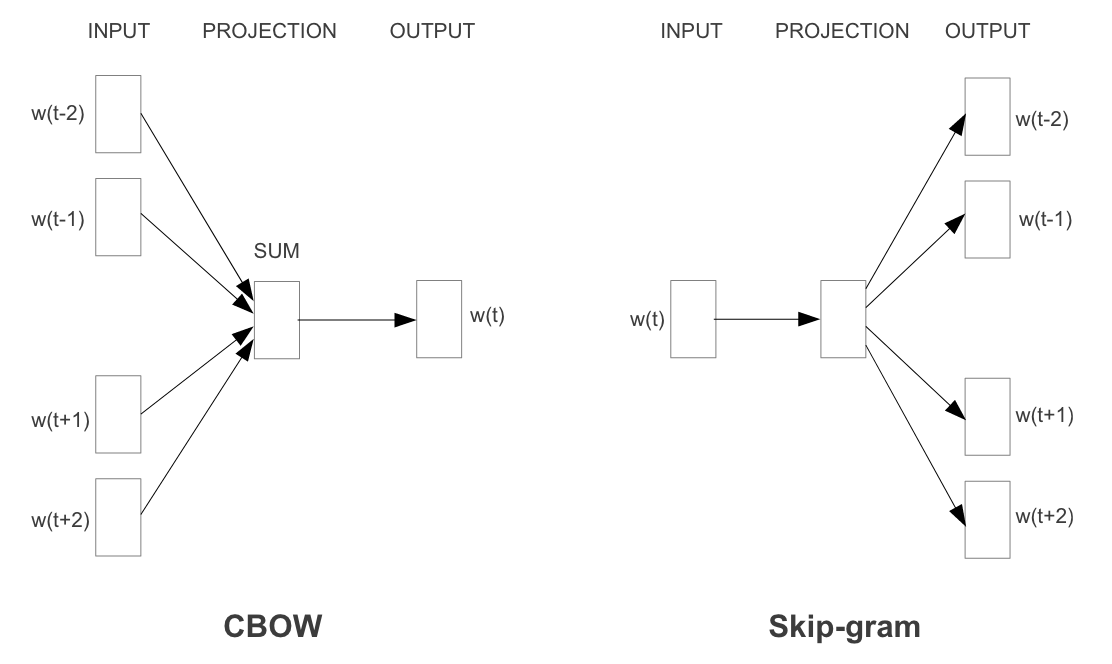
\includegraphics[width=0.7\textwidth]{screenshots/cbow_skipgram.png}
    \caption[\acl{CBOW} vs. Skip-Gram]{Learning Word Embeddings with \ac{CBOW} and Skip-Gram, illustration from \cite{MikolovEfficientEstimation2013}.
        Both models are predictive models: Whereas \ac{CBOW} predicts the target word $w_t$ from its context words $w_{t-2}, \dots, w_{t+2}$, the Skip-Gram model predicts the context words from the target word.}
    \label{fig:cbow-skipgram}
\end{figure}


\subsubsection*{FastText}

FastText, an extension of Word2Vec introduced by Bojanowski et al. \cite{BojanowskiEnrichingWord2017}, takes a more granular approach to word representation by treating each word as a bag of character n-grams. This allows FastText to capture the internal structure of words and the relationships between words sharing similar subword structures.

Although FastText employs the same Skip-Gram training objective as Word2Vec, it differs in how it computes the vectors for context or target words. Instead of using a single vector to represent a word, FastText uses the sum of the vectors of the character n-grams that compose the word. This can be mathematically represented as:

\begin{align}
    v_w = \sum_{g \in G_w} z_g \label{eq:fasttext}
\end{align}

where $v_w$ is the vector representation of word $w$, $G_w$ is the set of n-grams for word $w$, and $z_g$ is the vector representation of n-gram $g$.

As an example of word decomposition into character n-grams, the word \emph{where} is decomposed into the following character 3-grams: \texttt{<wh}, \texttt{whe}, \texttt{her}, \texttt{ere}, \texttt{re>}.
All n-grams for $3 \leq n \leq 6$ are considered by the default FastText model \cite{BojanowskiEnrichingWord2017}.
The decomposition of words into character n-grams allows FastText to handle rare and \ac{OOV} words more effectively than Word2Vec. Embeddings of unknown words are generated by summing the embeddings of their constituent subwords.


\subsubsection*{GloVe}

GloVe (Global Vectors for Word Representation), developed by Pennington et al. \cite{PenningtonGloveGlobal2014}, offers an alternative approach to word embedding distinct from methods like Word2Vec and FastText. While the latter models use predictive strategies that focus on individual local context windows during each training iteration, GloVe takes a count-based approach. It constructs a global word-word co-occurrence matrix by accumulating local context information across the entire corpus.

The unique strength of GloVe is its ability to combine both global corpus statistics and local semantic relationships into one unified model. To achieve this, it uses a weighted least squares regression objective function that operates directly on the co-occurrence counts matrix:

\begin{align}
    J = \sum_{i,j=1}^{V} f(X_{ij})(w_i^T \tilde{w}_j + b_i + \tilde{b}_j - \log X_{ij})^2 \label{eq:glove-objective-function}
\end{align}

In \Cref{eq:glove-objective-function}, $V$ denotes the vocabulary size, $w_i$ and $\tilde{w}_j$ represent the word vectors of word $i$ and context word $j$ respectively. $b_i$ and $\tilde{b}_j$ denote their respective biases. $X_{ij}$ quantifies the number of times word $j$ occurs in the context of word $i$ within a defined window size. Lastly, $f$ is a weighting function that diminishes the impact of both very rare and overly frequent co-occurrences.

Hence, the goal is to align the dot product of the word vectors ($w_i^T \tilde{w}_j$) and their biases ($b_i + \tilde{b}_j$) with the logarithm of the co-occurrence count ($\log X_{ij}$).
The word embeddings are learned by minimizing the sum of squared differences between these values, weighted by the factor $f(X_{ij})$.


\subsection{Contextual Embeddings} \label{sec:contextual-embeddings}

Unlike traditional static embeddings, which generate a single, fixed representation for each word regardless of its context, contextual embeddings produce a unique representation for each word based on its specific context within a sentence or a document.

As pointed out by Ruas et al. \cite{RuasMultisenseEmbeddings2019}, this advantage over static embeddings is particularly pronounced for polysemous words - words with multiple meanings. The author's methodology is rooted in integrating \ac{WSD} into the word embedding process. \ac{WSD} is a task in \ac{NLP} that identifies which sense of a word is used in a particular context. By incorporating \ac{WSD} into the word embedding generation process, the authors ensure that different senses of a word are accurately captured and represented.

Transformer-based models \cite{VaswaniAttentionAll2017} such as BERT \cite{DevlinBERTPretraining2019}, SciBERT \cite{BeltagySciBERTPretrained2019}, and Longformer \cite{BeltagyLongformerLongDocument2020} generate rich contextually-aware word embeddings by leveraging the Transformer architecture's self-attention mechanism.


\subsubsection*{Attention in Language Models}

The \emph{attention mechanism}, first introduced by Bahdanau et al. \cite{BahdanauNeuralMachine2016}, enables models to focus specifically on certain parts of an input sequence while generating each element of the output. This selective focus enables the model to detect relationships over long distances, irrespective of the actual distances between words. This represents a notable improvement over recurrent neural network (RNN) architectures, which process input sequences sequentially and struggle with long sequences due to the vanishing gradient problem.
Further, in contrast to recurrent neural networks, the attention mechanism allows the model to process the input sequence in parallel, leading to significant performance improvements \cite{VaswaniAttentionAll2017,AlammarIllustratedTransformer2018}.

In achieving this, the attention mechanism uses a process known as soft alignment between the input and output sequences. This process is particularly crucial for machine translation. In this scenario, the model learns to align the source and target sequences, focusing on pertinent parts of the source sequence as it generates each word in the target sequence. The alignment is realized by computing an attention score for each word in the source sequence. This score indicates the degree to which the model concentrates on that word while generating the target sequence.

The \emph{attention weight} $a_{ij}$ for a source word $j$ when generating a target word $i$ is determined as follows \cite{BahdanauNeuralMachine2016}:

\begin{align}
    a_{ij} = \frac{\exp(e_{ij})}{\sum_{k=1}^{T_x} \exp(e_{ik})} \label{eq:attention-weights}
\end{align}

In \Cref{eq:attention-weights}, $e_{ij}$ stands for the \emph{attention score} between target word $i$ and source word $j$, and $T_x$ represents the length of the source sequence. The attention score is typically computed as the dot product of the embeddings of the target and source words, although other scoring methods can also be applied. Once the attention scores are computed, they are passed to a softmax operation to ensure their sum equals one across the source sequence. The resulting attention weights $a_{ij}$ indicate the importance of the source word $j$ when generating the target word $i$. The attention weights are then used to compute a weighted sum of the source word embeddings, resulting in the final output of the attention mechanism.

The attention mechanism is illustrated in \Cref{fig:self-attention-bertviz} by Vig \cite{VigMultiscaleVisualization2019} on the example of BERT \cite{DevlinBERTPretraining2019}.

\begin{figure}[ht]
    \centering
    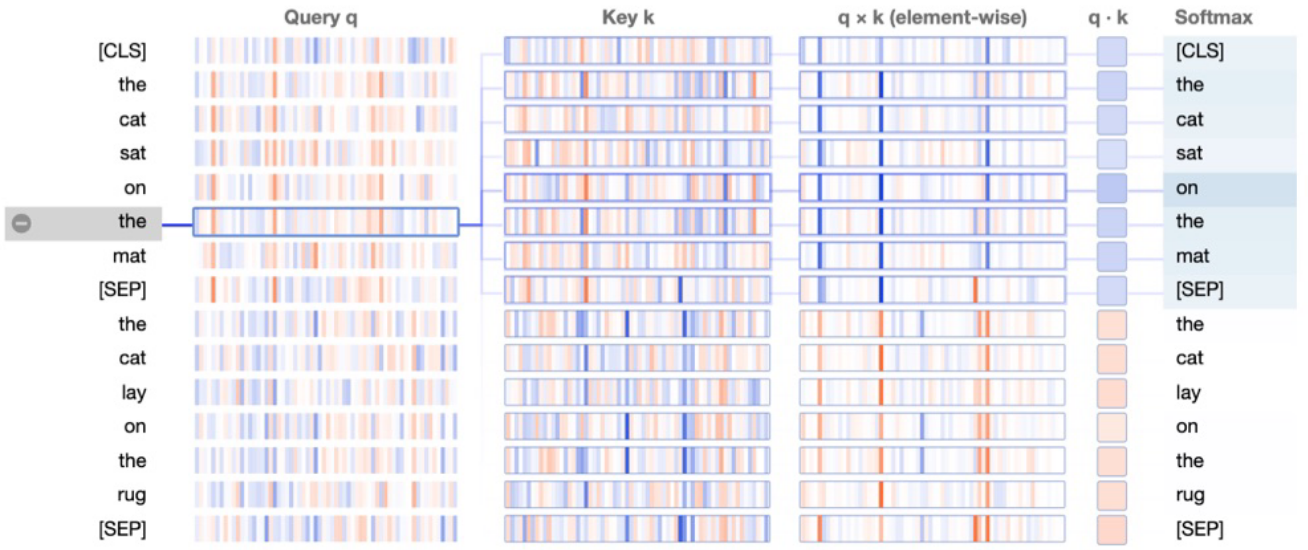
\includegraphics[width=\textwidth]{screenshots/self_attention_bertviz.png}
    \caption[The Attention Mechanism]{Visualization of the (self-) attention mechanism using BertViz \cite{VigMultiscaleVisualization2019}. The text tokens on the left represent the input sequence. Values of the query and key vectors are depicted as vertical bands of color. Blue represents positive values, while orange indicates negative ones. The color saturation is based on the value's magnitude. Lines connecting the query and key vectors represent attention weights. The line width corresponds to the magnitude of the attention weight.}
    \label{fig:self-attention-bertviz}
\end{figure}


\subsubsection*{The Transformer}

The Transformer model, introduced by Vaswani et al. \cite{VaswaniAttentionAll2017}, is the foundation of many of the recent advancements in \ac{NLP}. It was designed to handle sequence data efficiently and is thus well-suited for \ac{NLP} tasks. The cornerstone of the Transformer model is the self-attention mechanism. This is a particular implementation of the attention mechanism that is extended and modified to be applied not only between the source and target sequences but also within a single sequence. This allows the model to assign different weights to the words in a sentence when generating the embedding for a particular word, much like the attention mechanism described in the preceding section.

The self-attention mechanism associates each word in a sentence with a query, key, and value. These are derived from the input vector of the word and are instrumental in computing the attention score. The attention score between a query $Q_i$ and a key $K_j$ is calculated as the dot product of $Q_i$ and $K_j$, scaled by the inverse square root of the dimension of the key vectors to counteract the potential of the dot product growing large for high-dimensional vectors.

Formally, the scaled dot-product attention is defined as:

\begin{align}
    \text{Attention}(Q, K, V) & = \text{softmax}\left(\frac{QK^T}{\sqrt{d_k}}\right)V \label{eq:scaled-dot-product-attention}
\end{align}

where $d_k$ is the dimensionality of the key vectors, $Q$ is the matrix of query vectors, $K$ is the matrix of key vectors, and $V$ is the matrix of value vectors. The element-wise softmax function ensures the attention scores are normalized to sum to one.

The result of the softmax operation represents the attention weights in matrix form, showing the importance of each word in the context of the others. These attention weights are subsequently used to compute a weighted sum of the value vectors, encapsulating the relevant information from the sequence based on the learned attention scores.

Extending this mechanism, the Transformer model employs multi-head attention, wherein the model has multiple parallel attention layers referred to as \emph{heads}. Each head independently computes a different learned linear transformation of the input.
As illustrated in \Cref{fig:multi-head-attention}, the final output of the multi-head attention layer is the concatenation of the outputs of each head, followed by a linear transformation. This approach allows the model to capture various types of information and dependencies from the input sequence \cite{VigDeconstructingBERT2022a}.

\begin{figure}[ht]
    \centering
    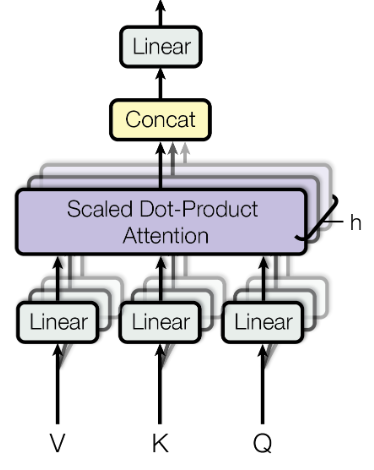
\includegraphics[width=0.3\textwidth]{screenshots/multi_head_attention.png}
    \caption[Multi-Head Attention]{Multi-head attention in the Transformer, illustration from \cite{VaswaniAttentionAll2017}.
        The input is transformed into query, key, and value vectors. Each of the $h$ attention heads transforms the input independently. The outputs of the heads are concatenated and linearly transformed to produce the final output.}
    \label{fig:multi-head-attention}
\end{figure}


\subsubsection*{BERT}

BERT (Bidirectional Encoder Representations from Transformers) is a Transformer-based model proposed by Devlin et al. \cite{DevlinBERTPretraining2019}. It builds upon the self-attention mechanism of the Transformer model to pre-train deep bidirectional representations from unlabeled text, conditioning on both left and right context in all layers. This bidirectionality allows BERT to learn context-rich word representations, a significant advancement over models which only consider unidirectional context \cite{McCormickBERTWord2019,AlammarIllustratedBERT2018}.

The pretraining process of BERT leverages two unsupervised tasks: \ac{MLM} and \ac{NSP}. In the \ac{MLM} task, about 15\% of the input tokens are randomly masked and the model is trained to predict these masked tokens based on the context provided by the non-masked tokens \cite{DevlinBERTPretraining2019}. This task encourages BERT to understand the context and relationships between words.

The \ac{NSP} task involves predicting whether a given sentence is the subsequent sentence of another sentence in the original text. During training, half of the inputs are pairs of sentences in which the second sentence is the subsequent sentence in the original document, while for the other half, a random sentence from the corpus is chosen as the second sentence. This task helps BERT understand relationships between sentences, a useful skill for many downstream \ac{NLP} tasks.

Once BERT is pretrained using a large corpus of text, it can be fine-tuned on downstream tasks using a relatively small amount of task-specific training data. The fine-tuning process involves minor adjustments to the pretrained parameters, allowing BERT to apply the general language understanding acquired during pretraining to the downstream task. This process is more efficient and requires less data than training a model from scratch, making BERT a highly effective model for a wide range of \ac{NLP} tasks.

\begin{figure}[ht]
    \centering
    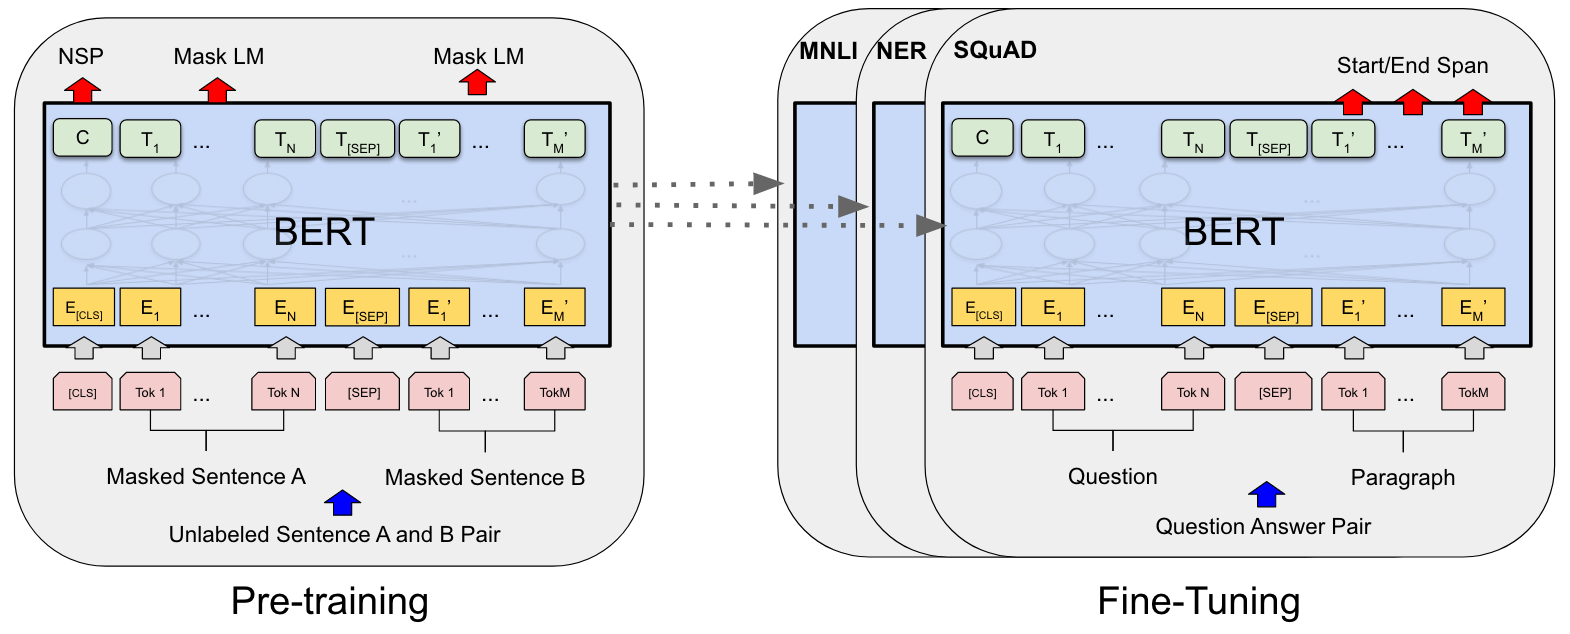
\includegraphics[width=\textwidth]{screenshots/bert.png}
    \caption[Pretraining and Fine-Tuning of BERT]{Pretraining and fine-tuning of BERT, illustration from \cite{DevlinBERTPretraining2019}.
        Left: BERT is pretrained on two unsupervised tasks: \acl{MLM} and \acl{NSP}. Right: The pretrained model can be fine-tuned for specific tasks, such as question answering, sentiment analysis, or named entity recognition, enhancing its downstream performance.}
    \label{fig:bert}
\end{figure}


\subsubsection*{SciBERT}

SciBERT, developed by Beltagy et al. \cite{BeltagySciBERTPretrained2019}, is a specialized variant of BERT that is designed to handle the unique language patterns and technical terminology found in scientific literature. This variant is especially effective for tasks related to scientific document classification, information extraction from scientific papers, and other tasks requiring comprehension of scientific text. Like BERT, SciBERT is pretrained using the \ac{MLM} and \ac{NSP} tasks. However, the training corpus is constructed from scientific papers, providing SciBERT with a stronger understanding of the language used in scientific literature.

The pretraining of SciBERT is drawn from the Semantic Scholar corpus, which includes approximately 1.14 million scientific papers spanning a wide range of disciplines.
WordPiece tokenization \cite{WuGoogleNeural2016} that breaks down words into subwords is used to handle \ac{OOV} words, which are quite common in the scientific domain due to the prevalence of unique terminologies, abbreviations, and symbols. This corpus and vocabulary construction strategy allows SciBERT to effectively handle the specific language patterns and technical jargon found in scientific literature.

The performance of SciBERT is tested on a range of \ac{NLP} tasks including sequence tagging (NER), sentence classification (textual entailment, sentiment analysis), and dependency parsing. The authors found that SciBERT outperformed BERT and achieved new state-of-the-art results on several tasks, particularly those involving scientific text \cite{BeltagySciBERTPretrained2019}.


\subsubsection*{Longformer}

The Longformer model, developed by Beltagy et al. \cite{BeltagyLongformerLongDocument2020}, aims to overcome the computational challenges of Transformer-based models like BERT when dealing with long documents. The self-attention mechanism in Transformer models has a computational complexity that grows quadratically with the length of the input sequence, making it inefficient for processing large-scale documents. Longformer addresses this issue by modifying BERT's self-attention mechanism to scale linearly with the input sequence length.
By integrating local and global attention mechanisms, Longformer offers an efficient solution for processing long documents, capturing their global context.

This novel self-attention mechanism, termed \emph{sliding window attention}, utilizes a fixed-size window that moves across the input sequence. Each token can only attend to other tokens within this window, effectively limiting the contextual scope of each token. This approach allows the model to manage computational resources efficiently, even when dealing with long sequences.

To enable the model to capture global context, Longformer integrates a limited number of globally attentive tokens into its architecture. These tokens can attend to the entire sequence, providing a mechanism for the model to gather information across the full length of the input. This feature is important for tasks that require a comprehensive understanding of the entire document, such as document classification and summarization.

The sliding window attention mechanism is contrasted from the traditional attention mechanism in \Cref{fig:sliding-window-attention} from Beltagy et al. \cite{BeltagyLongformerLongDocument2020}.
\Cref{tab:bert_longformer_tokenizer} compares the BERT and Longformer models in more detail including their tokenization processes.

\begin{figure}[ht]
    \centering
    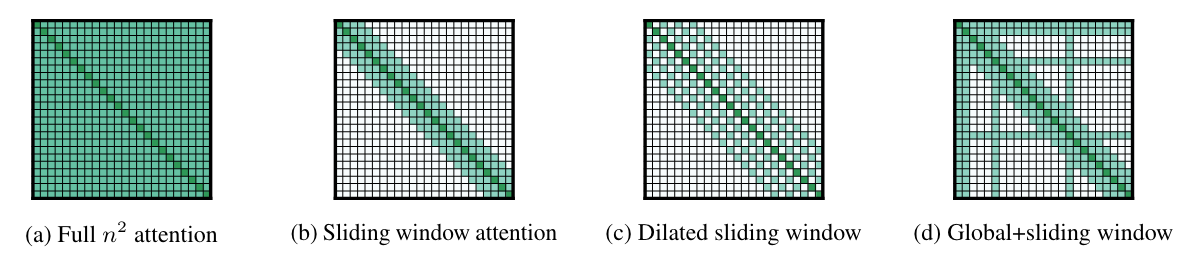
\includegraphics[width=\textwidth]{screenshots/sliding_window_attention.png}
    \caption[Sliding Window Attention]{Sliding window attention in the Longformer, as presented in \cite{BeltagyLongformerLongDocument2020}.
        Image a) demonstrates the standard self-attention mechanism where each token can attend to all other tokens.
        Image b) illustrates the sliding window attention mechanism where each token attends only to tokens within a fixed-size window.
        Image c) depicts the dilated sliding window attention where the tokens in the window are spaced with increasing gaps, allowing the model to attend to distant tokens without enlarging the window size.
        Image d) introduces global attention tokens that can interact with all other tokens in the sequence, capturing long-range dependencies.
    }
    \label{fig:sliding-window-attention}
\end{figure}


\subsection{Document Embeddings}

While word embeddings can capture the semantic content of individual words, they are limited in their ability to represent larger textual units such as whole documents. Document embeddings address this limitation by mapping entire documents to a high-dimensional vector space \cite{PalachyDocumentEmbedding2022}.

A straightforward method to derive document embeddings is by aggregating the embeddings of all individual words in the document.
Common approaches include averaging the word embeddings or calculating their dimension-wise maximum or sum. However, these techniques assume that all words contribute equally to the document's meaning and they do not consider the order of words. Further, the dimension-wise maximum is sensitive to outliers, whereas the sum is impacted by the document length.

To address these limitations, Kanakia et al. \cite{KanakiaScalableHybrid2019} propose a weighted average of word embeddings, computed as a normalized linear combination of the word vectors weighted by their TF-IDF scores \cite{SaltonTermWeighting1987}.
This method considers the significance of each word within the document.

Le and Mikolov \cite{LeDistributedRepresentations2014} extend the Word2Vec model by introducing \emph{Paragraph Vectors}, which are shared across all words in the paragraph. The paragraph vector is trained simultaneously with the word embeddings to predict a word from its context. After training, the paragraph vector is a semantic representation of the entire paragraph.
This model, often referred to as \emph{Doc2Vec}, has been used in diverse applications, including document classification \cite{OstendorffPairwiseMultiClass2020} and citation recommendation \cite{FarberHybridCiteHybrid2020,BhagavatulaContentBasedCitation2018}.

Ruas et al. \cite{RuasEnhancedWord2020} introduce two novel algorithms, which aim to enhance traditional word embeddings by leveraging multi-semantic representation through lexical chains. This method emphasizes the importance of the relationship between words in a sentence, capturing more about the underlying semantic content of a document than its individual words. By integrating semantic relations derived from lexical chains, document embeddings can be constructed from the most important correlated senses of the words in the document.

An alternative approach to document embeddings is proposed by Ostendorff et al. \cite{OstendorffSpecializedDocument2022}. Instead of representing a document as a single generic embedding, they represent it as multiple specialized embeddings, each capturing a distinct aspect of the document. This is achieved by considering the task, method, and dataset of the respective research papers as their aspects. The specialized embeddings are generated using various models, including FastText \cite{BojanowskiEnrichingWord2017}, SciBERT \cite{BeltagySciBERTPretrained2019}, and SPECTER \cite{CohanSPECTERDocumentlevel2020}.
Compared to traditional document embeddings, this method offers a more nuanced understanding of document similarity by effectively capturing the distinct aspects that make research papers similar.


\subsection{Document Similarity}

Once document embeddings are generated, it is possible to compute the similarity between documents.
There are numerous document similarity measures to choose from \cite{BriggsSemanticSearch2020}, and the choice of measure will depend on the specific task and the nature of the documents being compared. Two of the most popular measures are \emph{cosine similarity} and \emph{Jaccard similarity}.

\subsubsection*{Cosine Similarity}

Cosine similarity is calculated as the cosine of the angle $\theta$ between
two numerical document embedding vectors $\mathbf{a}$ and $\mathbf{b}$. In mathematical terms, this can be written as:

\begin{align}
    \text{cosine similarity} (\mathbf{a}, \mathbf{b})
    = \cos(\theta)
    = \frac{\mathbf{a} \cdot \mathbf{b}}{\|\mathbf{a}\|\|\mathbf{b}\|} \label{eq:cosine-similarity}
\end{align}

In \Cref{eq:cosine-similarity}, $\mathbf{a} \cdot \mathbf{b}$ is the dot product of $\mathbf{a}$ and $\mathbf{b}$, $\|\mathbf{a}\|$ and $\|\mathbf{b}\|$ are the magnitudes (Euclidean norms) of $\mathbf{a}$ and $\mathbf{b}$ respectively and $\theta$ is the angle between $\mathbf{a}$ and $\mathbf{b}$ \cite{SinghalModernInformation2001}.

Cosine similarity values range from -1 to 1.
As the cosine similarity between two vectors is closely linked to the correlation coefficient, the interpretation of these two measures is similar.
A value of 1 indicates perfect similarity, 0 means no similarity, and -1 represents perfect dissimilarity.
Cosine similarity is computationally efficient and is not influenced by document length. However, it might not be the best fit when the distribution of words is important, as it does not take into account the frequency or order of words.

\subsubsection*{Jaccard Similarity}

The Jaccard similarity coefficient \cite{JaccardEtudeDistribution1901} is another document similarity measure that works directly on the sets of words (tokens) in documents, not their document embedding vectors. It is the size of the intersection divided by the size of the union of the two word sets. This can be mathematically expressed as:

\begin{align}
    \text{Jaccard similarity} (A, B)
    = \frac{|A \cap B|}{|A \cup B|}
    = \frac{|A \cap B|}{|A| + |B| - |A \cap B|} \label{eq:jaccard-similarity}
\end{align}

where $|A|$ and $|B|$ are the cardinalities of the sets $A$ and $B$, respectively.

In \Cref{eq:jaccard-similarity}, $A$ and $B$ represent the sets of words in the two documents being compared.
In contrast to cosine similarity, the Jaccard similarity coefficient remains unaffected by word repetitions due to its use of sets containing unique elements. This makes it a good choice in cases where the presence or absence of words is more critical than their frequency or order, e.g. for short documents like titles and abstracts \cite{BreitingerAcademicLiterature2023}.


\subsubsection*{Advanced Similarity Measures}

Traditional document similarity measures such as cosine and Jaccard similarity may fall short in capturing the heterogeneous semantic relations between documents, as they do not consider the context in which similarity is evaluated. To address this, Ostendorff et al. \cite{OstendorffPairwiseMultiClass2020} propose a multi-class classification model for document pairs to determine semantic relations between documents.
Their results reveal that even complex relation classes yield promising performance, which is crucial for recommender systems and information retrieval applications.
They find that models that attend to both documents simultaneously, such as Siamese BERT \cite{DevlinBERTPretraining2019,ReimersSentenceBERTSentence2019} and Siamese XLNet \cite{YangXLNetGeneralized2020}, generally outperform traditional methods like AvgGloVe \cite{PenningtonGloveGlobal2014} and Doc2vec \cite{LeDistributedRepresentations2014}, which classify concatenated document vectors. However, these traditional methods still show reasonable performance, especially in scenarios where computational resources are limited.


\subsection{Applications in Paper Recommendation}

In academic paper recommendation, language models are often utilized to generate document embeddings for a given query paper and a set of potential candidate papers.
Based on these embeddings, the similarity between the query paper and each candidate paper is computed with a similarity measure such as cosine similarity. The candidate papers are then ranked based on their similarity score to the query paper with the highest-ranked papers being recommended to the user.
The details of this process including the choice of language model and the document sections used for generating embeddings can vary significantly among different approaches.

Bhagavatula et al. \cite{BhagavatulaContentBasedCitation2018} introduce a content-based strategy for citation recommendation. Existing citation recommendation systems often rely on metadata from the query documents, such as author names and publication venues. The authors note that during instances like the peer review process, this information might be missing. To address this issue, the authors propose a content-based method for citation recommendation that does not rely on metadata but instead uses the full text of the query document.
First, they embed the given query document into a vector space using Doc2Vec \cite{LeDistributedRepresentations2014}. Then, they identify papers with the highest cosine similarity as citation candidates. Finally, the authors train a discriminative model to predict the relevance of each candidate citation, which is then used to rank the candidates by predicted relevance.

Remaining in the context of paper citations, Cohan et al. \cite{CohanSPECTERDocumentlevel2020} introduce \emph{SPECTER}, a technique tailored for generating document embeddings within the scientific literature domain. SPECTER uses a transformer-based architecture that is pretrained with a citation prediction objective: given a citing paper and a list of candidate cited papers, it must identify the true cited paper. This objective allows the model to learn contextualized document representations from the citation graph.
SPECTER uses titles and abstracts, concatenated and preprocessed with SciBERT’s \cite{BeltagySciBERTPretrained2019} vocabulary, as its input.

Nascimento et al. \cite{NascimentoSourceIndependent2011} propose a content-based approach to generate recommendations using only a single research paper as input.
The authors propose a sequential strategy:
First, a set of candidate papers is generated with potential queries using terms from the input paper.
These queries are then submitted to existing web information sources that hold research papers.
Once a set of candidate papers for recommendation is retrieved, the framework applies content-based recommender algorithms to rank these candidates by using the paper title and abstract.

Mass and Roitman \cite{MassAdhocDocument2020} enhance ad-hoc document retrieval by leveraging the capabilities of pretrained models like BERT \cite{DevlinBERTPretraining2019} and GPT2 \cite{RadfordLanguageModels2018}. Their method uses weak supervision, leveraging unsupervised rankings from traditional retrieval methods and collecting pseudo-relevance feedback to curate training data. This data then serves to fine-tune the aforementioned pretrained models, with the objective of achieving enhanced retrieval performance. The models leverage the titles and abstracts of the papers to generate the embeddings.

Finally, Mohamed et al. \cite{A.MohamedBERTELMo2019} conduct a comparative evaluation of five widely used pretrained sentence encoders: USE \cite{CerUniversalSentence2018}, BERT \cite{DevlinBERTPretraining2019}, InferSent \cite{ConneauSupervisedLearning2018}, ELMo \cite{PetersDeepContextualized2018}, and SciBERT \cite{BeltagySciBERTPretrained2019}, in the context of research paper recommendation using only the paper titles. For each of the five models, the sentence embeddings of the input paper title and the candidate paper titles are calculated and their cosine similarity is used as a measure of semantic similarity. The authors observe that the efficacy of all models in recommending research papers, when considering only titles, is not on par with traditional techniques like BM25 \cite{RobertsonOkapiTREC31995}. However, when combined with BM25 in a hybrid approach, the performance improves.
In the hybrid setup, a linear combination of BM25 scores and semantic similarity scores is used to generate the final ranked recommendations.

Despite the widespread adoption of Transformer models, Beel et al. \cite{BeelResearchpaperRecommender2016} argue that models emphasizing lexical attributes over semantic ones remain the preferred choice for research paper recommendations. Their analysis discerned that $83\%$ of all content-based methods from 1998 to 2013 and $67\%$ of methods from 2014 to 2021 adopt TF-IDF as their principal weighting mechanism.
Nonetheless, the rise of \ac{LLMs} has sparked the interest in employing Transformer models for recommendation tasks. A discussion on the potential of \ac{LLMs} in recommender systems can be found in the Appendix.
